\section{Grupo fundamental}
Hemos de caracterizar diferentes espacios topológicos definiendo una
nueva propiedad llamada ``grupo fundamental''. Esta sera una invariante
del espacio bajo morfismos adecuados (a discutir mas adelante). Por
mientras hemos de enfocarnos que esta propiedad dependerá de la noción
de arcos admisibles en un espacio topológico. A continuación,
definiremos estos conceptos a adecuadamente.

{
\newcommand{\homRelAlt}{\stackrel{.}{\simeq}}
\subsection{Arcos y homotopías}
\begin{definicion}[Arco]
  Un arco en el espacio \(X\) es una función continua \(f : I \to X \)
  donde \(I = [0,1]\)
\end{definicion}
%% mariela: q1 ¿todo espacio 1-dimensional es homeomorfo a [0,1]?
%% no dije exactamente eso, un subconjunto convexo y acotado si lo es ,
%% pero debo de preguntar que se refiere
La definición tradicional es ligeramente mas general, cambiando que \(I\)
sea un subconjunto convexo acotado de un espacio unidimensional, pero
siempre podemos recuperar esta definición rescalando la distancia.

\begin{definicion}[Homotopía]
  Dados dos arcos \(f,g : I \to X\), diremos que \(f\) es homotópico a
  \(g\) si existe una función continua \(F : I \times I \to X \) tal que
  \[ \begin{matrix}
      F (x, 0) = f(x), & F (x, 1) = g(x)
     \end{matrix}
  \]
  Donde \(F\) sera llamada una homotopía entre \(f\) y \(g\). La
  existencia de dicha relación entre dos funciones sera denotada por \(f
  \homRelAlt g\).
\end{definicion}
\begin{figure}[h]
  \centering
  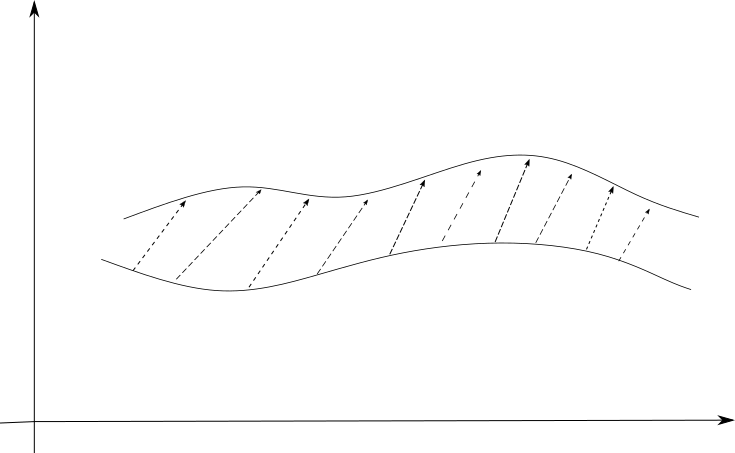
\includegraphics[scale=0.3]{./imagenes/homotopia.png}
  \caption{caracterización homotopía}
  \label{fig:homotopia-entre-funciones}
\end{figure}
Podemos pensar en el segundo argumento de una homotopía como el grado de
deformación entre dos funciones.
Si tratamos con arcos \(f,g : I \to X\) que posean los mismos puntos
iniciales y finales, es decir \(f(0) = g(0) = x_0, \; f(1) = g(1) =
x_1 \) podemos definir una relación homotópica ligeramente mas fuerte.

\begin{definicion}[Arco homotopía]
  \(f,g : I \to X\) son \emph{arco homotópicas} entre sí, si tienen los mismos
  puntos inicial y final \(x_0, x_1\) respectivamente y existe una homotopía entre
  ellos tal que cumpla
  \[
    \begin{matrix}
      F(s,0) = f(s), & F(s,1) = g(s) \\
      F(0,t) = x_0,  & F(1,t) = x_1
    \end{matrix}
  \]
  La existencia de esta relación entre dos funciones sera denotada por
  \(f \simeq g\).
\end{definicion}
% todo(slack) hacer algun dibujo de las homotopías entre las curvas
Una vez definida estas relaciones, una pregunta natural es si estas definen
una relación de equivalencia, ya que nos gustaría identificar clases de
curvas como elementos de alguna teoría algebraica. La respuesta es
afirmativa para ambas relaciones (el punto de inicio y final no juegan
un papel relevante). A continuación mostraremos que ``ser homotópicas''
es una relación de equivalencia.
\begin{teorema}
  \(\homRelAlt\) es una relación de equivalencia
\end{teorema}
\begin{proof}
  Hemos de probar que esta relación cumple la reflexividad, simetría y
  transitividad. Sean \(f,g,h : I \to X\) tres arcos arbitrarios.
  \begin{itemize}
  \item La reflexividad es directa pues la función \(F(x,t) = f(x)\) es
    una deformación continua de \(f\) a \(f\), por tanto \(f \homRelAlt
    f\).

  \item La simetría se obtiene de invertir el sentido de deformación de la
    homotopía original. Formalmente, dado \(f \stackrel{.}{\simeq} g\)
    tenemos una homotopía entre estas \((x,t) \mapsto F(x,t)\). A partir
    de aquí podemos definir
    \begin{equation}
      \label{eq:homotopy-simetry}
      (x,t) \mapsto \hat{F}(x,t) := F(x,1-t)
    \end{equation}
    con \(\hat{F}\) una homotopía entre \(g\) y \(f\). Por tanto \(g
    \stackrel{.}{\simeq} f\).

  \item La transitividad se obtiene a partir de de dividir \(I\) en dos
    intervalos donde se deformen individualmente cada homotopía al doble
    del grado. Formalmente dado \(f \stackrel{.}{\simeq} g\) y \(g
    \stackrel{.}{\simeq} h\) representadas por las homotopías \(F\) y
    \(G\) respectivamente, se define
    \[ FG(x,t) = \begin{cases}
        F(x,2t) & t \in [0,\frac{1}{2}] \\
        G(x,2t - 1) & t \in [ \frac{1}{2} , 1]
      \end{cases}
    \]
    Esta es una deformación continua claramente en \((x,t) \in I \times
    [0, \frac{1}{2}) \cup I \times (\frac{1}{2}, 1]\). La continuidad en
    \(I \times \{\frac{1}{2}\}\) proviene de la consistencia en dicho
    punto de ambas homotopías
    \[ F(x,2 \cdot \frac{1}{2}) = g(x) = G(x, 2 \cdot \frac{1}{2} - 1)\]
    lo que nos permite utilizar el \emph{lema del pegamiento}
    \cite[p.~108]{munkres} para obtener la continuidad de \(FG\).
    Obteniendo así \(f \stackrel{.}{\simeq} h\).
  \end{itemize}
\end{proof}

En análisis real, es común trabajar con conjuntos convexos. En arcos
sobre estos conjuntos, veremos una homotopía repetidamente llamada
homotopía de linea recta.
\begin{definicion}[Homotopía de linea recta]\label{def:homotopia-linea}
  Sean \(f,g : I \to X\) dos arcos arbitrarios y sea \(\mathcal C
  \subset X\) un subconjunto convexo. Si \(f(I),g(I) \subset \mathcal
  C\), entonces se define la homotopía de linea recta por
  \[ F(x,t) := (1-t) \cdot f(x) + t \cdot g(x) \]
\end{definicion}
\begin{acotacion}
  En la definición anterior, la continuidad de \(F\) se obtiene de ser
  una combinación convexa de funciones continuas \(f\) y \(g\). De que
  sea una combinación convexa se obtiene la importancia de que existe un
  conjunto \(\mathcal C \subset X\) que contenga a las imágenes.
\end{acotacion}

Con estas definiciones ya podemos empezar a hablar de \([f]\) clases
de equivalencia de funciones bajo una relación homotópica
\[ [f] = \{ g : I \to X \mid f \stackrel{.}{\simeq} g \} \]
Notar que la construcción es valida para las dos relaciones aunque por
nuestra meta de construir el grupo fundamental nos interesa
principalmente la relación arco homotópica, por razones a estudiar mas
adelante.

\subsection{Grupoide de arcos}
Si tenemos dos arcos continuos \(f,g\) tales que el punto final de \(f\)
sea el punto inicial de \(g\) podemos construir un camino continuo que
recorra \(f\) luego recorriendo \(g\). Esta idea es conocida formalmente
como el producto de dos arcos.

\begin{definicion}[Producto de arcos]
Para dos arcos \(f,g : I \to X\) tales que
\(f(1) = g(0)\), se define el producto \(f * g \)
\[ (f*g) (s) \coloneqq \begin{cases}
    f(2s) & s \in [0,\frac{1}{2}] \\
    g(2s - 1) & s \in [\frac{1}{2} , 1]
  \end{cases}
\]
la cual sigue siendo una funcion continua en virtud del lema del
pegamiento.
\end{definicion}

Esta construccion se puede reutilizar para clases
\emph{arco}-homotopicas \([f],[g]\) que compartan punto final e inicial
respectivamente para definir un producto de clases de equivalencia
\[ [f] * [g] \coloneqq [f * g]\]
El cual esta bien definido pues si \(f \simeq f' ,\ g \simeq
g'\) a traves de las homotopias \(F, G\) respectivamente, entonces
\[
  H(s,t) = \begin{cases}
    F(2s,t) & s \in [0, \frac{1}{2}] \\
    G(2s - 1, t) & s \in [\frac{1}{2} , 1]
  \end{cases}
\]
Es la homotopia que relaciona a los arcos que sean homotopicos a
\(f*g\). Esta ademas es continua en virtud otra vez del lema del pegamiento.

\paragraph{} Con esta operacion binaria, una pregunta a hacerse es si
\((\mathcal C (I , X)/\simeq , (*))\) tiene posee estructura de
grupoide, esto equivale a cumplir 3 propiedades
\begin{enumerate}
\item \textbf{Asociatividad} Si \([f] * ([g] * [h])\) esta definido entonces
  tambien lo debe estar \(([f] * [g]) * [h]\) y ademas deben coincidir.
\item \textbf{Identidades izquierda y derecha} Para todo \([f]\) con
  \(x_0, x_1\) puntos inicial y final respectivamente, debe de
existir elementos \([k_{x_0}], [k_{x_1}]\) tales que
\[ \begin{matrix}
    [f] * [k_{x_1}] = [f] & & [k_{x_0}] * [f] = [f]
  \end{matrix}
\]
\item \textbf{Inverso} Para todo \([f]\) clase de arcos con \(x_0, x_1\)
  puntos inicial y final respectivamente debe de existir un elemento
  \([f^{-1}]\) que cumpla
\[ \begin{matrix}
    [f] * [f^{-1}] = [k_{x_0}] & & [f^{-1}] * [f] = [k_{x_1}]
  \end{matrix}
\]
\end{enumerate}
Para probar esto necesitamos primero definir a nuestros candidatos de
\(k_{x_0}, k_{x_1}, f^{-1}\) ademas de algunas funciones auxiliares,
iniciando por los mapeos constantes e identidad en \(I \to I\)
\[ \begin{matrix}
     e_0 : & I \to I & e_0(t) \coloneqq 0 \\
     e_1 : & I \to I & e_1(t) \coloneqq 1 \\
     i :   & I \to I & i(t) \coloneqq t \\
     \bar{i} : & I \to I & i(t) \coloneqq 1 - t
   \end{matrix}
   \]
Ademas, para todo arco \(f : I \to X \), el elemento \(f^{-1} : I \to X \) esta
definido (en el espiritu de \eqref{eq:homotopy-simetry}) por
\[ f^{-1} (s) \coloneqq f (1 - s) \]
Por ultimo, para todo \(x \in X \) se define la curva
constante\footnote{\(k\) por \emph{konst}}
\begin{align*}
  k_x : &I \to X \\
        &t \mapsto x
\end{align*}
Con esto podemos afrontar la demostración
\begin{proof}
Se procedera en orden \(2 \to 3 \to 1\) con lemas en medio. Sea \(f : I
\to X\) el representante de la clase \([f]\). sean \(x_0, x_1\) los
puntos inicial y final de \(f\) respectivamente.

\paragraph{(2).} Dados \(i,e_1\) arcos en \(I\) definidos anteriormente,
es claro que \(i * e_1\) es tambien un arco (continuo) en \(I\); mas aun,
ya que \(I = [0,1]\) es convexo, se tiene \(i * e_1 \simeq i\) con la
homotopia de la linea recta entre estos denotada por \(C\).

Tambien conocemos que la composición de funciones continuas es
continua, de lo cual podemos decir que dada una homotopia \(H : I \times
I \to I\) la composicion \( f \circ H : I \times I \to X\) es una homotopia.

Por otro lado, necesitamos conocer como se comporta la composicion con
respecto a nuestro producto \((*)\), para esto tenemos el siguiente lema
\begin{lema}[Distributividad de la composicion sobre producto]
\label{lema:dist-composicion-producto}
\[\forall a,b : I \to I,\ \forall f : I \to X,\ f \circ (a * b) = (f
\circ a) * (f \circ b) \]
\end{lema}
\begin{proof}
  \[ f \circ (a*b) (s) =
    \begin{cases}
      f (a(2s)) & s \in [0,\frac{1}{2}] \\
      f (b(2s - 1)) & s \in [\frac{1}{2} , 1]
    \end{cases}
    = (f \circ a) * (f \circ b) (s)
  \]
\end{proof}

Luego esto nos permite afirmar en especifico que
\[ f \circ i \simeq f \circ (i * e_1) = (f \circ i) * (f \circ e_1) \]
en virtud de la homotopia
\[ f \circ C : I \times I \to X \]
Por tanto
\begin{equation}\label{eq:homequiv2.1}
[f \circ i] = [f \circ (i * e_1)] = [(f \circ i) * (f \circ e_1)]
\end{equation}
Si tomamos este ultimo termino, sabemos que por definicion
\begin{equation}\label{eq:homequiv2.2}
[(f \circ i) * (f \circ e_1)] = [(f \circ i)] * [(f \circ e_1)]
\end{equation}
y es claro tambien que
\[
  \begin{matrix}
    f \circ i = f & f \circ e_1 = k_{x_1} \\
  \end{matrix}
\]
\begin{equation}\label{eq:homequiv2.3}
[(f \circ i)] * [(f \circ e_1)] = [f] * [k_{x_1}]
\end{equation}
juntando
\eqref{eq:homequiv2.1},\eqref{eq:homequiv2.2},\eqref{eq:homequiv2.3} nos
muestra que \([k_{x_1}]\) es la identidad por la derecha. Podemos
hacer un proceso analogo para \([k_{x_0}]\) como identidad por la
izquierda, asi probando (2).

\paragraph{(3).} De manera similar a la pregunta anterior, notar que \(i,
\bar{i}\) definidos anteriormente cumplen
\[ i * \bar{i} \simeq e_0 \]
por la homotopia de linea recta en el espacio \(I\) que es convexo.
Utilizando el lemma \eqref{lema:dist-composicion-producto} tenemos que
\[ [f * f^{-1}] = [f \circ (i * \bar{i})] = [f \circ e_0] = [k_{x_0}] \]
\[ \implies [f] * [f^{-1}] = [k_{x_0}] \]
De manera analoga se prueba la inversa por la izquierda.

\paragraph{(1).}
Por definicion, tenemos que las diferentes asociaciones nos resultan en
diferentes representates de clase
\[
  \begin{matrix}
    (f * g) * h \, (t) =
    \begin{cases}
      f (4t), & t \in [0, \frac 1 4] \\
      g (4t - 1), & t \in [\frac 1 4, \frac 1 2] \\
      h (2t - 1), & t \in [\frac 1 2, 1] \\
    \end{cases} &
    f * (g * h) \, (t) =
    \begin{cases}
      f (2t), & t \in [0, \frac 1 2] \\
      g (4t - 2), & t \in [\frac 1 2, \frac 3 4] \\
      h (4t - 3), & t \in [\frac 3 4, 1] \\
    \end{cases}
  \end{matrix}
\]
Sea \(T : I \to I\) definida por
\[ T (t) :=
  \begin{cases}
    2t & t \in [1 , \frac 1 4] \\
    t + \frac 1 4 & t \in [\frac 1 4, \frac 1 2] \\
    \frac t 2 + \frac 1 2 & t \in [\frac 1 2, 1]
  \end{cases}
\]
\(T\) es una funcion continua por el lema del pegamiento. Por ser \(I\)
un dominio convexo, se tiene que \(i \simeq T\), luego
\[ [(f * g) * h] = [\big( (f * g) * h \big) \circ i] = [\big( (f * g) *
  h \big) \circ T ] = [f * (g * h)] \]
\end{proof}


\subsection{Grupo fundamental}
Sobre nuestros arcos tenemos una estructura de grupoide y no de grupo
porque no siempre podemos hacer coincidir los puntos inicial y final de
las diferentes clases de arcos. Si nos fijáramos en un solo punto \(x_0
\in X\) tal que todas los arcos \(f : I \to X\) cumplieran que la igualdad
\[ f(0) = x_0 = f (1) \]
Entonces las propiedades que demostramos anteriormente nos dirían que el
espacio \((\mathcal C \left( I , X \right) / _\simeq , \left( *
\right))\) es un grupo algebraico.
\begin{definicion}[Grupo fundamental]
  Sea \(X\) un espacio topológico y \(x_0 \in X\) un punto. La colección
  \[ \pi_1 (X,x_0) = \{ [f] \mid f : I \to X
     ,\ f(0)=f(1)=x_0,\ f \text{ continua}\}\]
  \[ [f] := \{ g : I \to X \mid f \simeq g\}\]
  junto con el producto de caminos \((*)\) forman el llamado
  \textbf{grupo fundamental} \((\pi_1(X,x_0), (*))\)
\end{definicion}

Nuestro interés es mostrar que para un espacio dado, su grupo
fundamental es una invariante topológica. Esto quiere decir que dado dos
espacios puntuados \((X,x_0)\) e \((Y,y_0)\) homeomorfos, debe de
existir un respectivo isomorfismo de grupos entre \(\pi_1(X,x_0)\) y
\(\pi_1(Y,y_0)\). Para esto debemos recordar que un isomorfo entre
grupos es un homomorfismo, inyectivo y sobreyectivo.
\begin{definicion}[Homomorfismo] \label{def:homomorfismo}
  Sean \((G,(*)), (G'', (\cdot))\) dos grupos algebraicos. \(F : G \to
  G'\) es un homomorfismo entre grupos si y solo si
  \[ \forall x,y \in G,\ F (x * y) = F(x) \cdot F(y)\]
\end{definicion}
% Mariela me dijo que esto es un corolario, no se si si quiera es
% necesario.
\begin{observacion}
  \[ e \text{ es identidad de } G \implies F(e) \text { es identidad de } G' \]
\end{observacion}

\begin{ejemplo}[Grupo fundamental: \(\mathbb{R}^2 \backslash
  \{(1,1)\}\). ] \label{ex:R2-11}
Para mostrar la intuición detrás de la definición, utilizaremos como
ejemplo un espacio relativamente sencillo de visualizar. Hemos de
caracterizar todas la curvas cerradas que inicien en un punto
arbitrario, que denotaremos por \(x_0\). Sea \(f : I \to \mathbb{R}^2 -
\{(1,1)\}\) un camino arbitrario, con dicho punto inicial, tendremos
tres grandes alternativas para de su clasificación.
\begin{figure}[h]
  \centering
  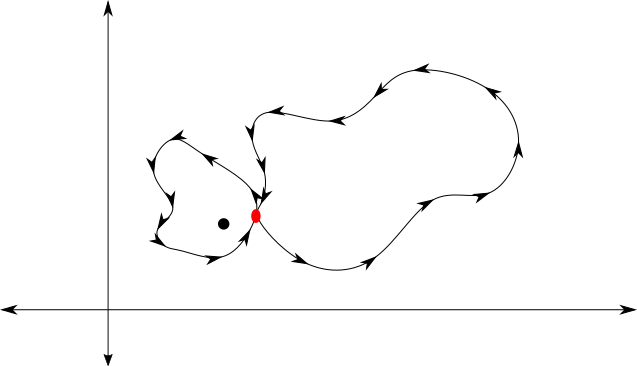
\includegraphics[scale=0.5]{./imagenes/R2-punto.png}
  \caption{\(R^2\) sin el punto \((1,1)\) en negro. Origen en rojo. }
  \label{fig:R2-sin-punto}
\end{figure}
\begin{itemize}
\item La curva denotada por \(f\) puede estar contenida en un subconjunto
  convexo de \(R^2 - \{(1,1)\}\). De esta manera, la curva pertenece a la
  homotopía de la linea recta dada por la definición
  \ref{def:homotopia-linea} bajo la función
  \[ L (t,\lambda) = \lambda f (t) - (1 - \lambda) k_{x_0} (t)\]
  Por lo tanto en este caso, \(f \in [k_{x_0}]\).
  %% TODO: mariela pide que cambie convexo, no entiendo bien
\item La curva \(f\) no puede ser contenida en un subconjunto convexo de
  \(R^2 - \{ (1,1)\}\). Esto solo puede suceder si la curva \(f\)
  encerrara al punto \((1,1)\), de manera que la relación \(\lambda x +
  (1 - \lambda) y\) no seria valida para algunos \(\lambda, x, y\). Por
  tanto \(f \not \in [k_{x_0}]\), así que denotaremos a la clase de
  equivalencia a la que pertenezca como \([\mathtt{F}^1]\).
\item La curva \(f\) encierra a \((1,1)\) \(2\) veces. Podemos definir dos
  caminos \(g_1, g_2\) tales que \(f = g_1 * g_2\) (modulo re-escalamiento
  en parámetros) y que \(g_1, g_2 \in \mathtt [F ^1]\). Esto nos diría que
  \( f \in [\mathtt F ^1] * [\mathtt F ^1] =: [\mathtt F ^2]\). Este
  procedimiento puede generalizar para todos los naturales.
% \item La curva \(f\) encierra a \(x_0\) \(2\) veces. Dado que cada vez
%   que lo encierra, esa curva (hasta ese momento) es homotópica a
%   \([\mathtt F ^1]\), tenemos que \(f\) es isometrica a \( [\mathtt F
%   ^1] * [\mathtt F ^1] =: [\mathtt F ^2]\). Esto se puede generalizar
%   para todos los naturales.
\end{itemize}
Así intuitivamente vemos que para este tenemos las clase de
equivalencias \([k_{x_0}], [\mathtt F ^1], [\mathtt F ^2], \dots \) con
la propiedades algebraicas
\[ [k_{x_0}] * [\mathtt F ^n] = [\mathtt F ^n] * [k_{x_0}]\]
\[ [\mathtt F ^m]  * [\mathtt F ^n] = [\mathtt F ^{n + m}]\]
En efecto, estos elementos son bajo isomorfismo de grupo equivalentes a
el grupo \((\mathbb{Z}, +)\). Por tanto diremos que este es el grupo
fundamental de \(R^2 - \{(1,1)\}\).
\end{ejemplo}

Cabe notar que esta no es una demostración formal, no se ha demostrado
que estas son todas alternativas posibles de curvas, de lo cual depende
todo nuestro argumento. Mas adelante daremos una demostración formal de
que esta intuición es la correcta, pero por ahora sirve como marco
conceptual del objeto que estamos estudiando.

\subsection{Importancia punto de origen}
En el ejemplo anterior se vio que el punto \(x_0\) la verdad no
jugaba ningún papel importante, su única misión era identificar el
origen de los caminos. En espacios como el anterior, la importancia de
la elección se ve reducida puesto que este es arco-conexo, en estos
espacio \(\forall a,b \in X\), con \(X\) un espacio topológico a
estudiar, existe un camino \(\alpha : I \to X\) tal que \(\alpha (0) =
a,\ \alpha (1) = b\). Si nuestro espacio \(X\) no fuera arco-conexo,
caemos en la disyuntiva de elegir un punto apropiado que represente
``suficientemente'' al espacio, en la definición de su grupo
fundamental. Dada que la motivación de definir en primer lugar el grupo
fundamental provenía de establecer una \emph{invariante} topológica,
hace dudar que la parametrizacion en cuanto a punto base del grupo
fundamental indique que procedemos por buen camino
%todo(slack): buscar papers de grupo fundamental de conjuntos conexos y
%no arco conexos

Aun en espacios arco-conexos seguimos declarando el punto base con
respecto al cual derivamos su grupo fundamental. Para ver con mas
claridad el por que, primero debemos probar que en efecto, en espacios
arco-conexos el grupo fundamental no depende del punto de partida. En
este resultado, nos sera muy útil el concepto de conjugación de un
camino.
\begin{definicion}[Conjugado de un camino] \label{def:conjugada}
  Sea \(\alpha : I \to X\) un camino en \(X\) tal que \(\alpha (0) =
  x_0,\ \alpha(1) = x_1\). La función definida por
  \begin{align*}
    \hat \alpha : \pi (X, x_0) &\longrightarrow \pi (X, x_1) \\
    [g] &\longmapsto [ \overline{\alpha} * g * \alpha ]
  \end{align*}
  con \(\overline \alpha\) el camino inverso de \(\alpha\) (ver ecuacion
  \eqref{def:camino-inverso}) es llamada la conjugada de \(\alpha\).
\end{definicion}
\begin{teorema} \label{not:alpha-hat}
  Sea \(x_0 , x_1 \in X\) puntos de un espacio arco conexo, sean \(\pi
  (X, x_0), \pi (X, x_1)\) dos grupos fundamentales de \(X\)
  parametrizados por estos puntos, entonces estos dos grupos son isomorfos
\end{teorema}
\begin{proof}
  Por ser \(X\) arco-conexo, existe \(\alpha : I \to X\) camino
  continuo, tal que \(\alpha (0) = x_0,\ \alpha (1) = x_1\). Se define
  la función conjugada de \(\alpha\) por \(\hat \alpha\).
  Esta función, esta bien definida puesto que \(\forall g \in \pi (X,
  x_0),\ \overline{\alpha} * g * \alpha \) es continua (en virtud de \(*\)).
  Por definición y reducción se tiene
  \[ \overline{\alpha} (t) = \alpha (1 - t)\]
  \[\big(\overline{\alpha} * g * \alpha \big) (0) = \alpha (1 - 0) = x_1
    = \alpha (1) = \big(\overline{\alpha} * g * \alpha \big) (1)\]

  \paragraph{\(\hat \alpha\) es homomorfismo:} Se procede por
  definición. Por un lado, al mapear la identidad de \(k_{x_0} \in \pi
  (X, x_0) \), tenemos por simple calculo las siguientes igualdades
  \begin{align*}
    \hat \alpha ([k_{x_0}])
                 &= [\overline{\alpha} * k_{x_0} * \alpha] \\
                 &= [\overline{\alpha}] * [k_{x_0} * \alpha] \\
                 &= [\overline{\alpha}] * [\alpha] \\
                 &= [\overline{\alpha} * \alpha] \\
                 &= [k_{x_1}] \\
  \end{align*}
  Por otro lado, si \(u,v \in \pi (X, x_0) \), tenemos la siguiente
  reducción del producto
  \begin{align*}
    \hat \alpha ([u] * [v]) &= [\overline{\alpha} * u * v * \alpha] \\
    &= [\overline{\alpha} * u * k_{x_0} * v * \alpha] \\
    &= [\overline{\alpha} * u * \alpha * \overline{\alpha} * v * \alpha] \\
    &= [\overline{\alpha} * u * \alpha ] * [ \overline{\alpha} * v * \alpha] \\
    &= \hat \alpha (u) * \hat \alpha (v)
  \end{align*}

  \paragraph{\(\hat \alpha\) es inyectiva y sobreyectiva.} La inyectividad es
  clara, pues si \([u],[v] \in \pi (X, x_0),\ [u] \not \simeq [v]
  \implies [\overline{\alpha}] * [u] * [\alpha] \not \simeq
    [\overline{\alpha}] * [v]
  * [\alpha]\). Para ver la sobreyectividad, notemos que \(\forall [k] \in
  \pi (X, x_1) \), siempre existe \( [\alpha * k * \overline{\alpha}]\) tal
  que
  \[ \hat \alpha ([\alpha * k * \overline{\alpha}]) = [\overline{\alpha}
    * \alpha * k * \overline{\alpha} * \alpha] = [k]\]
  Por tanto \(\hat \alpha\) es un isomorfismo de grupos.
\end{proof}
En la prueba anterior, la existencia del camino \(\alpha\)
parametrizaba que tipo de isomorfismo \(\hat \alpha\) construimos.
La elección de punto bases
\(x_0, x_1\) nos permite hablar de la existencia de único o múltiples
isomorfismos entre grupos fundamentales \(\pi (X, x_0), \pi (X, x_1) \)
dependientes de la cantidad de caminos entre \(x_0\) y \(x_1\) que
existan. Esto es un tema importante a considerar, puesto que existe una
caracterización de \(\pi (X, x_0) \) como grupo \emph{Abeliano}, que depende de
la cantidad de estos isomorfismos.
\begin{teorema}
  Sean \(x_0, x_1 \in X\) puntos en un espacio arco-conexo. El grupo
  \(\pi (X, x_0) \) es Abeliano si y solo si \(\forall \alpha, \beta\)
  caminos (distintos) entre \(x_0\) y \(x_1\), se cumple que \(\hat
  \alpha \equiv \hat \beta\), con \(\hat \alpha, \hat \beta\) los
  conjugados de los caminos respectivos.
\end{teorema}
\begin{proof}
  Primero, dado que \(\pi (X, x_0)\) es
  Abeliano, esto significa que \(\forall [f],[g] \in \pi (X, x_0),\ [f]
  * [g] = [g] * [f]\). Sean \(\alpha, \beta\) caminos entre \(x_0,x_1\)
  fijos pero arbitrarios. Para mostrar que \( \hat \alpha = \hat \beta\),
  debemos mostrar que para todo argumento estas funciones coinciden. Sea
  \([f] \in \pi (X, x_0) \) un argumento fijo pero arbitrario. Dado que
  \(\alpha * \overline{\beta} * \beta \simeq \alpha \), se tiene que
  \[ \hat \alpha = \widehat{(\alpha * \overline{\beta} * \beta)}\]
  Luego por definición se cumplen la siguientes reducciones
  \[ \hat \alpha ([f]) = \widehat{(\alpha * \overline{\beta} * \beta)} ([f]) =
    [\overline{\beta}] * [\beta * \overline{\alpha}] * [f] * [\alpha *
    \overline{\beta}] * [\beta]
  \]
  Donde \([\alpha * \overline{\beta}] \in \pi (X, x_0) \), por lo tanto
  podemos aplicar conmutatividad con \([f] \in \pi (X,x_0)\) obteniendo la
  siguiente expresión
  \[
    [\overline{\beta}] * [\beta * \overline{\alpha}] * [\alpha *
    \overline{\beta}] * [f] * [\beta] = [\overline{\beta}] * [f] * [\beta] =
    \hat \beta ([f])
  \]
  probando así lo buscado.

  En el converso, sean \([f],[g] \in \pi (X, x_0) \) fijos pero
  arbitrarios. Dado que \(\alpha\) es camino entre \(x_0\) y \(x_1\), se
  tiene que \(f * \alpha\) también es camino entre \(x_0\) y \(x_1\).
  Por hipótesis, tenemos en particular para estos caminos, que se cumple
  la relación
  \begin{align*}
    \widehat{\left( f * \alpha \right)} ([g]) &= \hat{\alpha} ([g]) \\
    [\overline{(f * \alpha)} * g * (f * \alpha) ] &= [\overline{\alpha}
      * g * \alpha] \\
    [\overline{\alpha} * \overline{f} * g * f * \alpha ] &=
      [\overline{\alpha} * g * \alpha] \\
    [\overline{\alpha}] * [\overline{f}] * [g] * [f] * [\alpha] &=
      [\overline{\alpha}] * [g] * [\alpha] \\
    [\overline{f}] * [g] * [f] &= [g] \\
    [g] * [f] &= [f] * [g], \qquad \forall [f],[g] \in \pi (X, x_0) \\
  \end{align*}

  \begin{acotacion}
    Aquí se esta utilizando la notación \( [\alpha]\) para clase de
    equivalencias no necesariamente pertenecientes al grupo fundamental
    \(\pi (X, x_0)\).
  \end{acotacion}
\end{proof}

En resumen si sabemos que \(\pi (X, x_0)\) es \emph{Abeliano}, esto equivale a
decir que \(\forall \alpha,\beta\) caminos entre \(x_0, x_1\), se tiene
que existe un \emph{único} isomorfismo entre \(\pi (X,x_0) \) y \( \pi
(X,x_1)\), pues \(\hat \alpha = \hat \beta\). Anteriormente, teníamos la
existencia de posiblemente múltiples isomorfismos entre \(\pi (X, x_0)
\) y \(\pi (X, x_1) \). Si no podemos parametrizar los isomorfismos
entre distintos puntos bases de un grupo fundamental, perdemos esta
caracterización de grupo fundamental Abeliano, pues perdemos la capacidad
de contar cuantos isomorfismos existen.

\subsection{Invariante topológica}
Nuestra meta original era mostrar que el grupo fundamental es una
invariante topológica de un espacio. Esto es que dados dos
espacios topológicos \(X,Y\) tales que \(x_0 \in X,\ y_0 \in Y\), si
existe un homeomorfismo (función biyectiva continua con inversa
continua)
\begin{align*}
  h : (X, x_0) &\longrightarrow (Y, y_0) \\
  x_0 &\longmapsto h(x_0) = y_0
\end{align*}
entre \((X, x_0)\) y \((Y, y_0)\) entonces existirá un isomorfismo de
grupos
\[ h_{*} : \pi (X, x_0) \longrightarrow \pi (Y, y_0) \]
entre \(\pi (X, x_0)\) y \(\pi (Y, y_0)\). Existe una manera natural de
construir dicho isomorfismo mediante la definición de cierto
homomorfismo, al cual mostraremos a continuación
\begin{definicion}[Homomorfismo inducido] \label{def:homomorfismo-inducido}
  Sea \(h : (X, x_0) \longrightarrow (Y, y_0)\) un morfismo de
  espacios topológicos puntuados. La función
  \begin{align*}
    h_* : \pi (X, x_0) &\longrightarrow \pi (Y, y_0) \\
    [f] &\longmapsto [h \circ f]
  \end{align*}
  es denominada el homomorfismo inducido por \(h\) entre \(\pi (X,
  x_0)\) y \(\pi (Y, y_0)\).
\end{definicion}
\begin{teorema} \label{thm:morfismo-homomorfismo}
  Para \(h : (X, x_0) \to (Y, y_0)\) un morfismo entre espacios
  puntuados, \(h_* : \pi (X, x_0) \to \pi (Y, y_0)\) es un homomorfismo
\end{teorema}
\begin{proof}
  Primero mostraremos que este homomorfismo esta bien definido. Esto
  equivale a mostrar que esta basado en \(y_0\) y que es
  independiente de representante de clase de \([f]\). Lo primero lo
  vemos pues por hipótesis se sabe que \(h
  (x_0) = y_0\) y que \([f] \in \pi (X, x_0)\) lo que implica que \(h_* ([f]) =
  [h \circ f] \in \pi (Y, y_0)\) esta basado correctamente. Para la
  independencia de representante de clase, tomemos \(f_1, f_2 \in [f]
  \in \pi (X, x_0)\), por definición existe una homotopía \(H\) entre
  \(f_1, f_2\) por pertenecer a la misma clase de equivalencia. Luego la
  función \(h \circ H\) es una homotopía entre \(h \circ f_1\) y \(h \circ
  f_2\) y  por tanto
  \[ h_* \left( [f_1] \right) = h_* \left( [ f_2 ] \right)\]

  Nos falta probar de que cumple la
  ecuación de un homomorfismo dadas por la definición
  \ref{def:homomorfismo}. Esto se ve por definición
  \ref{def:homomorfismo-inducido} de \(h_*\) y por el
  lema \ref{lema:dist-composición-producto} de composición sobre el
  producto, obtenemos las siguientes igualdades
  \[
    h_{*} ([f * g])
    = [h \circ (f * g)]
    = [(h \circ f) * (h \circ g)]
    = h_{*} ([f]) * h_{*} ([g])
  \]
  obteniendo así lo buscado.
\end{proof}
Si sabemos que \(h\) es además un homeomorfismo, tenemos el siguiente
teorema
\begin{teorema} \label{thm:homoemorfismo-isomorfismo}
Si \(h : (X, x_0) \to (Y,y_0)\) es un homeomorfismo, entonces \(h_{*} :
\pi (X, x_0) \to \pi (Y, y_0)\) es un isomorfismo de grupos.
\end{teorema}
\begin{proof}
Por el teorema anterior, solo hemos de probar que si \(h\) un
homeomorfismo entonces \(h_*\) es inyectivo y sobreyectivo.
\begin{itemize}
  \item Para la inyectividad, nos basamos en que \(h\) ya es un
  homeomorfismo. Sea \([f], [g] \in \pi (X, x_0)\) tales que \(h_* ([f])
  = h_* ([g])\), por definición esto es equivalente a la siguiente
  ecuaciones
  \begin{align*}
    &~ [h \circ f] = [h \circ g] \\
    &\iff h \circ f \simeq h \circ g \\
    &\iff f \simeq g \quad (h \text{ biyectiva}) \\
    &\iff [f] = [g]
  \end{align*}

  \item Para la sobreyectividad, dado que \(h^{-1} :
  (Y,y_0) \to (X, x_0)\) también es un homeomorfismo, para todo \([u] \in
  \pi (Y, y_0) \) se tiene que \(h_{*} ([h^{-1} \circ u]) = [u]\).
\end{itemize}
\end{proof}

Saber que el grupo fundamental es una invariante sin duda es útil
desde un punto de vista topológico, pero la idea de poder reflejar
estructura algebraica entre dos representaciones de un objeto y que esta
se preserve bajo morfismos es útil en su propia ley. En efecto, la
teoría que estudia este fenómenos es llamada teoría de categorías e
históricamente los grupos fundamentales dieron inicio al estudio de
estas.
\begin{definicion}
  Una categoría \(\mathcal C\) consiste una tripleta \(( \mathbf {Obj},
  \mathbf {Mor}, (\circ))\), donde
  \begin{itemize}
    \item \(\mathbf {Obj}\) corresponde a una clase\footnote{Clase en el
      sentido de teoría de conjuntos Neumann–Bernays–Gödel} de objetos.
    \item \(\mathbf {Mor}\) corresponde a una clase de morfismos entre
      elementos de \(\mathbf {Obj}\), tal que para todo \(A \in
      \mathbf {Obj}\) existe un único morfismo identidad \( \mathcal i
      _A : A \to A, \ i_A \in \mathbf{Obj}\).
    \item \((\circ)\) es una operación composición entre morfismos
      asociativa .
  \end{itemize}
\end{definicion}
\begin{definicion}
  Sean \(\left( \mathscr{C} , (\circ) \right), \left(\mathscr D ,
  (\star) \right) \) dos categorías con sus respectivos operadores
  composición. Un functor \(F : \mathscr C \to \mathscr D\) es un mapeo
  tal que cumple las siguientes propiedades
  \begin{itemize}
  \item \(\forall X \in \mathbf{Obj}(\mathscr C),\ F(X) \in \mathbf{Obj} (\mathscr D)\)
  \item \(\forall f \in \mathbf{Mor} (\mathcal C)\) morfismo de \(X,Y
    \in \mathbf{Obj} (\mathcal C)\) , se
    debe cumplir que \(F (f)\) tenga la siguiente forma
    \[ F(f) : F(X) \to F(Y),\ F(f) \in \mathbf{Mor}
      (\mathcal D) \]
    Mas aun, el morfismo identidad \(i_A\) para \(A \in
    \mathbf{Obj} (\mathcal C)\) debe cumplir la ecuación \(F (i_A) =
    i_{F(A)}\)
  \item Si \(f,g \in \mathbf{Mor}(\mathcal C)\) son morfismos tales que
    \(f \circ g \in \mathbf{Mor} (\mathcal C)\), entonces
    \[ F(f \circ g) = F(f) \star F(g) \]
  \end{itemize}
\end{definicion}
% TODO: imagen de functor mapeando
Es decir, un functor es una función entre categorías que preserva la
estructura de morfismos en la categoría inicial en la estructuras de
morfismos en la categoría de llegada. Nosotros hemos ya construido
nuestro primer functor, donde nuestras categorías inicial y de llegada son
\[ \mathcal C = \mathscr{Top}_* ,  \quad \mathcal D
  = \mathscr{Grp} \]
con \(\mathcal {Top}_*\) la categoría con objetos espacios topológicos
puntuados con morfismos funciones continuas entre ellos (mapeando punto de
orígenes) y \(\mathscr{Grp}\) la categoría de grupos con homomorfismo entre
grupos con composición usual. Para especificar formalmente nuestro
functor \(F\), debemos especificar tanto el mapeo de los elementos como
el de los morfismos. Estos están dados por las siguientes ecuaciones
\begin{align*}
  F : \mathscr{Top}_* &\longrightarrow \mathscr{Grp} \\
  \forall (A, a_0) \in \mathbf{Obj} \left( \mathscr{Top}_* \right),\
    &F(A) \coloneqq \pi (A, a_0) \\
  \forall f \in \mathbf{Mor} \left( \mathscr{Top}_* \right),\ &F(f) \coloneqq
    f_*
\end{align*}
Los morfismos \(f\) de \(\mathscr{Top}_*\) cumplen por teorema
\ref{thm:morfismo-homomorfismo} que \(f_*\) es un homomorfismo. Viendo
específicamente los homeomorfismos de \(\mathscr{Top}_*\),
el teorema \ref{thm:homoemorfismo-isomorfismo} nos dice que en la
categoría de llegada estos son isomorfismos de grupos. Es decir este
functor preserva isomorfismos.
}